This layer is the mount that controls the release and locking of the tool.


\subsection{Mount Layer Hardware}
There is a 3D printed housing for this layer using PLA plastic. It contains the magnet as well as a insertion point for the tool being used by the robotic arm.  A wire connecting the magnet to the UR5's arm is located here. (There is an internal wire that connects to the control box). The tool is assumed to have a metal contact for the magnet to attach to.

\subsection{Mount Layer Operating System}
N/A

\subsection{Mount Layer Software Dependencies}
N/A

\subsection{Connector}
This interface is an 8 pin connection point that uses a Lumberg RKMV 8-354 cable.  This is how the control box sends a signal to the magnet to provide it power.

\begin{figure}[h!]
	\centering
 	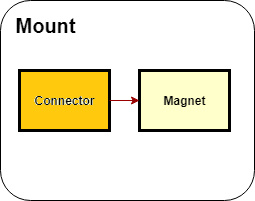
\includegraphics[width=0.60\textwidth]{images/Mount_Layer_Connector}
 \caption{Mount Layer Connector diagram}
\end{figure}

\subsubsection{Connector Subsystem Hardware}
The 8 pin connection is standard connection in robots uses to provide various signals to connected equipment. In this case a 12V voltage drop is provided to the magnet.

\subsubsection{Connector Subsystem Operating System}
N/A

\subsubsection{Connector Subsystem Software Dependencies}
N/A

\subsubsection{Connector Subsystem Programming Languages}
N/A

\subsubsection{Connector Subsystem Data Structures}
N/A

\subsubsection{Connector Subsystem Data Processing}
N/A

\subsection{Magnet}
This is the subsystem that makes contact directly with the tool being used and locks or releases it depending on signals from the connector subsystem.

\begin{figure}[h!]
	\centering
 	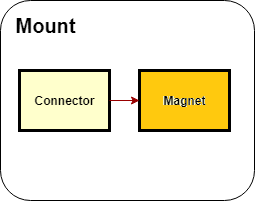
\includegraphics[width=0.60\textwidth]{images/Mount_Layer_Magnet}
 \caption{Mount Layer Connector diagram}
\end{figure}

\subsubsection{Magnet Subsystem Hardware}
The 12V magnet of this system has a payload of about 11 pounds and is the contact point for the metallic end of the tool's handle/shaft.

\subsubsection{Magnet Subsystem Operating System}
N/A

\subsubsection{Magnet Subsystem Software Dependencies}
N/A

\subsubsection{Magnet Subsystem Programming Languages}
N/A

\subsubsection{Magnet Subsystem Data Structures}
N/A

\subsubsection{Magnet Subsystem Data Processing}
N/A
